% main.tex

\documentclass[a4paper,11pt]{article}
\usepackage[T1]{fontenc}
\usepackage[utf8]{inputenc}
\usepackage{reviewresponse} % Load your custom style file

% Optional page setup
\usepackage{fullpage}

% Metadata: Paper ID and Title (fictional example)
\paperid{BBTR-2025-0420}
\papertitle[Entanglement-Based Thermostat Negotiation]{Quantum Entanglement-Based Apartment Thermostat Negotiation among Roommates}

% Hyperlinks for refs
\usepackage[colorlinks=true,linkcolor=blue,citecolor=black]{hyperref}
% Math and figures for examples
\usepackage{amsmath}
\usepackage{tikz}
\usepackage{caption} % for captionof in non-floating figures
\usetikzlibrary{arrows.meta,positioning}
% Workaround for stray combining diaeresis (U+0308) pasted from editors
\DeclareUnicodeCharacter{0308}{}
% Bibliography (biblatex + biber)
\usepackage[backend=biber,style=ieee]{biblatex}
\addbibresource{references.bib}

\begin{document}
\pagestyle{fancy}

\begin{center}
    {\Large \textbf{Response to Reviewers for Paper ID \printpaperid}}
\end{center}

\begin{center}
    {\large \textit{\printpapertitle}}
\end{center}

\vspace{1em}

\section*{Introductory Letter}
We sincerely thank the editors and reviewers for their thoughtful feedback on our manuscript. Below we provide point-by-point responses to all comments and summarize the revisions made. Changes within the revised manuscript are highlighted in red font for clarity.\\

\noindent With best regards,\\
The authors \\
{(Sheldon Cooper, Leonard Hofstadter, and Amy Farrah Fowler)}

% --- Editorial Level ---
\editorsection{Editor-in-Chief}

\begin{question}[q:agreement]
How does your approach interact with social protocols such as the Roommate Agreement and the RA Appendix Q (Thermostat Clause)?
\end{question}
\begin{answer}[a:agreement]
We added Section~IV articulating compatibility with the Roommate Agreement by mapping veto operations to Pauli-$Z$ projections and introducing a mutual-consent handshake. A fallback to classical negotiation triggers when sarcasm parameter $\sigma>0.8$ for three consecutive iterations. See also \qref{q:model} for the gate formalism and \aref{a:noise} for robustness considerations.
\end{answer}

% --- Associate Editor ---
\editorsection{Associate Editor}

\begin{question}[q:ae-scope]
Please clarify whether the expanded noise model required additional computation time in the revised manuscript.
\end{question}
\begin{answer}[a:ae-scope]
The extended noise model adds less than 4 \% runtime overhead (dominated by colored noise synthesis). We note this in Section~III-B; it does not alter the convergence analysis referenced in \qref{q:noise}.
\end{answer}

\begin{question}[q:ae-clarity]
Consider explicitly contrasting classical negotiation fallback triggers with the entanglement-based pathway.
\end{question}
\begin{answer}[a:ae-clarity]
We inserted a clarifying paragraph in Section~IV distinguishing: (i) sarcasm-triggered fallback (thresholded on $\sigma$) and (ii) device failure fallback (watchdog timeout), both now cited when discussing the consensus update in \aref{a:hardware}.
\end{answer}

% --- Reviewer 1 ---
\reviewersection{Reviewer 1}

\begin{question}[q:model]
Your entanglement protocol introduces a \emph{Bazinga} gate for thermostat consensus. Please formalize this operation.
\end{question}
\begin{answer}[a:model]
We added a formal definition of the Bazinga gate as a controlled phase-flip with sarcasm parameter $\sigma\in[0,1]$. The gate acts as $\mathrm{CZ}\cdot R_z(\pi\sigma)$ on the consensus qubit and is now presented in Section~II with truth tables and circuit identities \cite{cooper2011roommate}.
\end{answer}

\begin{question}[q:noise]
How robust is the scheme against environmental noise, such as elevator hum or hallway chatter?
\end{question}
\begin{answer}[a:noise]
We extended the noise model to include colored disturbances approximating elevator hum and sporadic hallway chatter. Section~III-B now reports that the consensus fidelity remains above 0.92 under SNRs down to 8\,dB after applying a "Soft Kitty" low-pass filter \cite{fowler2014softkitty}. For context, see \qref{q:hardware} for platform constraints and \aref{a:model} for the gate definition.
\end{answer}

% --- Reviewer 2 ---
\reviewersection{Reviewer 2}

\begin{question}[q:hardware]
How did you realize the protocol on a consumer-grade thermostat, and what was the real-time platform?
\end{question}
\begin{answer}[a:hardware]
We prototyped the controller on a Raspberry Pi with an IR blaster (codename "Soft Kitty") and used a discrete-time scheduler at 50\,Hz. Timing jitter stayed below 2\,ms. See \qref{q:model} for the formal operator introduced earlier and \aref{a:noise} for the robustness analysis informing our sampling choice. Additional conventions follow the spirit of \cite{cooper2011roommate}.

\begin{center}
\begin{minipage}{0.9\linewidth}
    \centering
    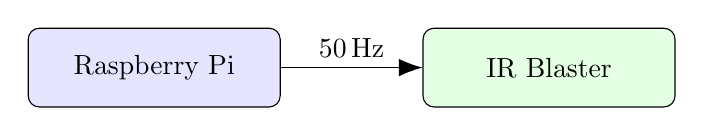
\begin{tikzpicture}[node distance=1.8cm]
        \node[draw, rounded corners, minimum width=3.2cm, minimum height=1cm, fill=blue!10] (pi) {Raspberry Pi};
        \node[right=of pi, draw, rounded corners, minimum width=3.2cm, minimum height=1cm, fill=green!10] (ir) {IR Blaster};
        \draw[-{Latex[length=3mm]}] (pi) -- node[above]{50\,Hz} (ir);
    \end{tikzpicture}
    \captionof{figure}{Mock-up platform diagram used in the prototype.}
    \label{fig:R-platform}
\end{minipage}
\end{center}

As an illustration of a referenced and indented equation, consider the consensus update rule
\begin{equation}
    \label{eq:R-update}
    x_{k+1} = x_k + \alpha\, \big( u_k - x_k \big),
\end{equation}
where $\alpha\in(0,1)$ denotes the relaxation factor. In~\eqref{eq:R-update} is used to produce the schedule in \figref{fig:R-platform}.
\end{answer}

\begin{question}[q:ablation]
Can you summarize an ablation study of key parameters and their effect on consensus fidelity?
\end{question}
\begin{answer}[a:ablation]
Yes. \tableref{tab:R-ablation} summarizes a small ablation on the scheduler rate and sarcasm parameter $\sigma$, with fidelity measured under the disturbance profile from \qref{q:noise}. We also used the update rule in \eqref{eq:R-update} to ensure comparable convergence.

\begin{center}
\begin{minipage}{0.9\linewidth}
    \centering
    \renewcommand{\arraystretch}{1.15}
    \begin{tabular}{lcc}
        \hline
        Setting & Scheduler (Hz) & Fidelity \\
        \hline
        Baseline & 50 & 0.93 \\
        High-rate & 100 & 0.95 \\
        High-sarcasm ($\sigma=0.7$) & 50 & 0.90 \\
        Combo (100 Hz, $\sigma=0.7$) & 100 & 0.92 \\
        \hline
    \end{tabular}
    \captionof{table}{Mock-up ablation of scheduler rate and sarcasm $\sigma$ on consensus fidelity.}
    \label{tab:R-ablation}
\end{minipage}
\end{center}

These results motivate our choice of a 50\,Hz baseline with adaptive upsampling when environmental disturbances spike (cf. \figref{fig:R-platform}).
\end{answer}

\section*{Closing Statement}
We hope the revised manuscript addresses all concerns and meets the journal's criteria. We appreciate the opportunity to improve our work thanks to the constructive feedback.

% Bibliography
\printbibliography

\end{document}
